%%
% F19 CSCI 466 Networks
%
% Finite State Machine (FSM) for 
% Trivia Server Proxy
%
% Phillip J. Curtiss, Associate Professor
% pcurtiss@mtech.edu, 406-496-4806
% Department of Computer Science, Montana Tech
%%
\documentclass[10pt]{article}
\usepackage[utf8]{inputenc}
\usepackage[T1]{fontenc}
\usepackage[margin=.75in]{geometry}
\usepackage{amsmath,amssymb,amsfonts}
\usepackage{tikz}
\usetikzlibrary{calc,arrows,automata,shapes.multipart,positioning}

\begin{document}
\pagestyle{empty}

 \begin{center}
    \textbf{F19 CSCI 466 - Trivia Server FSM}
    \vfill
    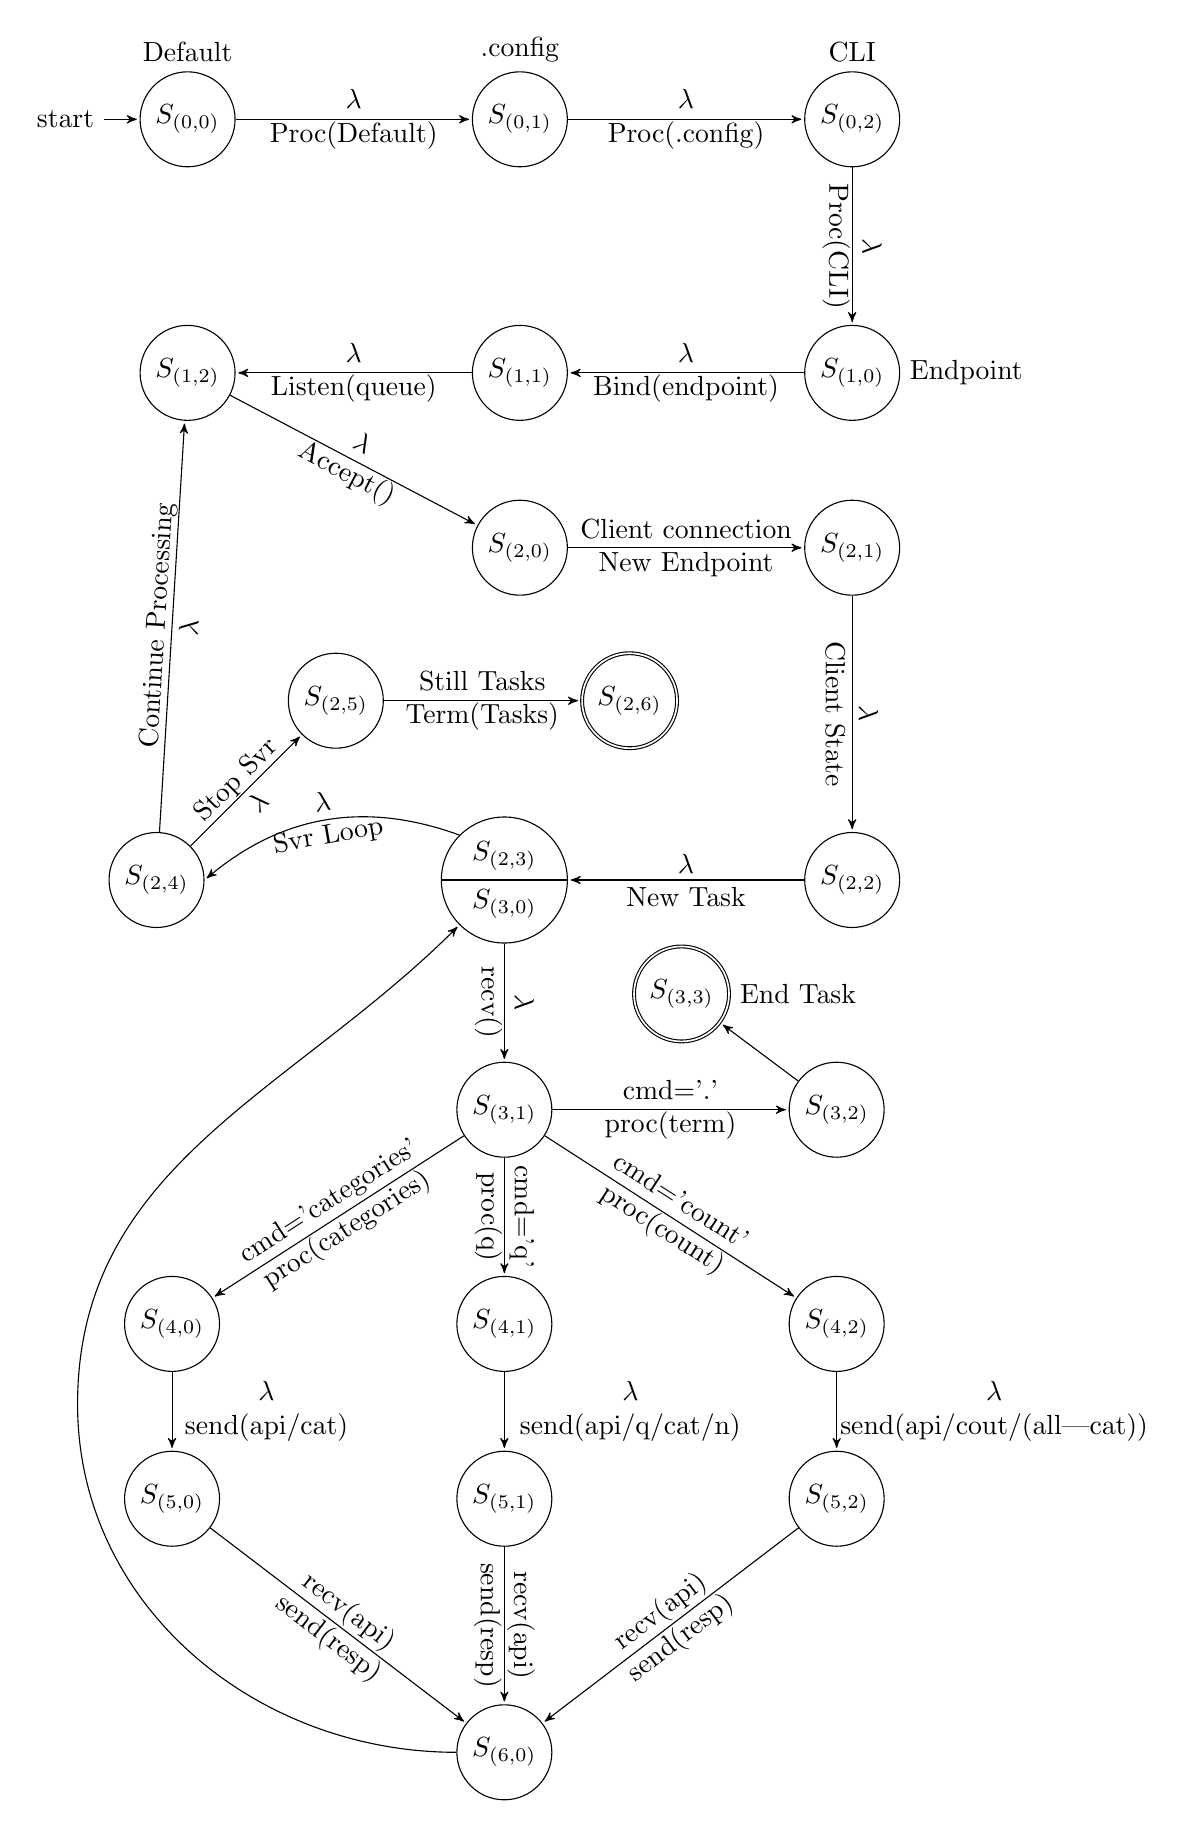
\begin{tikzpicture}[
        >=stealth', shorten > = 1pt,
        node distance=3cm
    ]

%%
% Initial Connection Steps for Establising 
% Server Connect - socket, bind, listen
    \node (s00) [initial,state,label=above:{Default}] {$S_{(0,0)}$};
    \node (s01) [state,right=of s00,label=above:{.config}] {$S_{(0,1)}$};
    \node (s02) [state,right=of s01,label=above:{CLI}] {$S_{(0,2)}$};
    \node (s10) [state,below=2cm of s02,label=right:{Endpoint}] {$S_{(1,0)}$};
    \node (s11) [state,left=of s10] {$S_{(1,1)}$};
    \node (s12) [state,left=of s11] {$S_{(1,2)}$};
    \path[->]
        (s00) edge node[align=center] {$\lambda$\\ Proc(Default)} (s01)
        (s01) edge node[align=center] {$\lambda$\\ Proc(.config)} (s02)
        (s02) edge node[align=center,sloped] {$\lambda$\\ Proc(CLI)} (s10)
        (s10) edge node[align=center] {$\lambda$\\Bind(endpoint)} (s11)
        (s11) edge node[align=center] {$\lambda$\\Listen(queue)} (s12);
%%
% Server Loop:
% Accept, new endpoint, Client State,  New Task
% New Task services each connected client
    \node (s20) [state,below=1cm of s11] {$S_{(2,0)}$};
    \node (s21) [state,right=of s20] {$S_{(2,1)}$};
    \node (s22) [state,below=of s21] {$S_{(2,2)}$};
    \node (s23) [draw,circle split,left=of s22] {$S_{(2,3)}$ \nodepart{lower} $S_{(3,0)}$};
    \node (s24) [state,left=of s23] {$S_{(2,4)}$};
    \node (s25) [state,above right=2cm of s24] {$S_{(2,5)}$};
    \node (s26) [accepting,state,right=2.5cm of s25] {$S_{(2,6)}$};
    \path[->]
        (s12) edge node[align=center,sloped] {$\lambda$\\Accept()} (s20)
        (s20) edge node[align=center] {Client connection\\New Endpoint} (s21)
        (s21) edge node[align=center,sloped] {$\lambda$\\Client State} (s22)
        (s22) edge node[align=center] {$\lambda$\\New Task} (s23)
        (s23.north west) edge [bend right] node[align=center,sloped] {$\lambda$\\Svr Loop} (s24.east)
        (s24) edge node[align=center,sloped] {Continue Processing\\$\lambda$} (s12)
        (s24) edge node[align=center,sloped] {Stop Svr\\$\lambda$} (s25)
        (s25) edge node[align=center] {Still Tasks\\Term(Tasks)} (s26);
%%
% Connected Client:
% Terminate upon command dot '.'
    \node (s31) [state,below=1.5cm of s23] {$S_{(3,1)}$};
    \node (s32) [state,right=of s31] {$S_{(3,2)}$};
    \node (s33) [accepting,state,above left=0.6cm and 1.1cm of s32,label=right:{End Task}] {$S_{(3,3)}$};
    \path[->]
        (s23) edge node[align=center,sloped] {$\lambda$\\recv()} (s31)
        (s31) edge node[align=center] {cmd='.'\\proc(term)} (s32)
        (s32) edge (s33);
%%
% Connected Client:
% count, categories, q command processing
% Received command from user and send to opentdb web service api
    \node (s41) [state,below=1.5cm of s31] {$S_{(4,1)}$};
    \node (s40) [state,left=of s41] {$S_{(4,0)}$};
    \node (s42) [state,right=of s41] {$S_{(4,2)}$};
    \node (s50) [state,below=1cm of s40] {$S_{(5,0)}$};
    \node (s51) [state,below=1cm of s41] {$S_{(5,1)}$};
    \node (s52) [state,below=1cm of s42] {$S_{(5,2)}$};
    \path[->]
        (s31) edge node[align=center,sloped] {cmd='q'\\proc(q)} (s41)
        (s31) edge node[align=center,sloped] {cmd='categories'\\proc(categories)} (s40)
        (s31) edge node[align=center,sloped] {cmd='count'\\proc(count)} (s42)
        (s40) edge node[align=center,xshift=1.2cm] {$\lambda$\\send(api/cat)} (s50)
        (s41) edge node[align=center,xshift=1.6cm] {$\lambda$\\send(api/q/cat/n)} (s51)
        (s42) edge node[align=center,xshift=2cm] {$\lambda$\\send(api/cout/(all|cat))} (s52);
%%
% Receive the response from the opentdb, process into a standard string builder
% send the response to the end user
% go back to loop - to retrieve next command from user
    \node (s60) [state,below=2cm of s51] {$S_{(6,0)}$};
    \path[->]
        (s50) edge node[align=center,sloped] {recv(api)\\send(resp)} (s60)
        (s51) edge node[align=center,sloped] {recv(api)\\send(resp)} (s60)
        (s52) edge node[align=center,sloped] {recv(api)\\send(resp)} (s60);
    \draw[->]
        (s60) to[out=west,in=south] ($(s50)+(-1.2,1.2)$) to[out=north,in=south west] (s23);

    \end{tikzpicture}
 \end{center}

\end{document}
